\documentclass{article}
\usepackage{fancyhdr}
\usepackage{caption}
\usepackage{tikz}
\usepackage{slashbox}
\pagestyle{fancy}
\lhead{Modo ejemplo}
\rhead{Proyecto II IC6400}
\begin{document}
\section*{Resultados del modo de ejemplo}
\subsection*{I. Descripción del problema}
Se tienen 6 llaves diferentes (A, B, C, D, E y F), cada una de las cuales tiene una probabilidad diferente de ser buscada. El objetivo es construir un \'arbol de b\'usqueda binario a partir de estas llaves, de forma que el tiempo de b\'usqueda promedio sea el menor posible. Para esto se emple\'o un algoritmo de programaci\'on din\'amica y un algoritmo greedy.

\subsection*{II. Datos del problema}
Los datos utilizados se resumen en la siguiente tabla:

\begin{table}[ht]
\centering
\begin{tabular}{r|l|l|l|l|l|l}
Llave & A & B & C & D & E & F  \\\hline
Probabilidad & 0.15 & 0.14 & 0.21 & 0.10 & 0.11 & 0.29
\end{tabular}
\label{datos}
\end{table}

\subsection*{III. Programación Dinámica}
A continuaci\'on se muestran las tablas generadas por el algoritmo de programaci\'on din\'amica para encontrar el \'arbol \'optimo. Adem\'as, se muestra el \'arbol resultante.

Tiempo de ejecución: 0.000003 segundos.
\begin{table}[ht]
\centering
\begin{tabular}{c|ccccccc}
\backslashbox{$i$}{$j$} & 0 & 1    & 2    & 3    & 4    & 5    & 6    \\ \hline
1 & 0.00 & 0.15 & 0.43 & 0.86 & 1.13 & 1.45 & 2.24 \\
2 & & 0.00 & 0.14 & 0.49 & 0.69 & 1.01 & 1.80 \\
3 & & & 0.00 & 0.21 & 0.41 & 0.73 & 1.41 \\
4 & & & & 0.00 & 0.10 & 0.31 & 0.81 \\
5 & & & & & 0.00 & 0.11 & 0.51 \\
6 & & & & & & 0.00 & 0.29 \\
7 & & & & & & & 0.00 \\

\end{tabular}
\caption{Matriz A generada por el algoritmo de programación din\'amica}
\label{A}
\end{table}

\begin{table}[ht]
\centering
\begin{tabular}{c|cccccc}
\backslashbox{$i$}{$j$} & 1    & 2    & 3    & 4    & 5    & 6    \\ \hline
1 & 1 & 1 & 2 & 3 & 3 & 3 \\
2 & & 2 & 3 & 3 & 3 & 3 \\
3 & & & 3 & 3 & 3 & 5 \\
4 & & & & 4 & 5 & 6 \\
5 & & & & & 5 & 6 \\
6 & & & & & & 6 \\

\end{tabular}
\caption{Matriz R generada por el algoritmo de programación din\'amica}
\label{R}
\end{table}

\begin{figure}[ht]
\centering
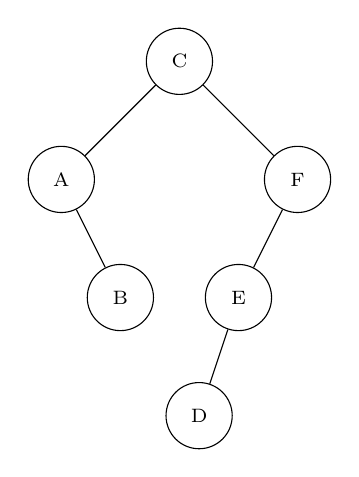
\begin{tikzpicture}[
every node/.style = {minimum width = 3em, draw, circle},
level/.style={sibling distance={3cm/max(1,#1)}}
]
\scriptsize
\node {C}
child {
node {A}
child[missing]
child{
node {B}
}
}
child {node {F}
child{
node {E}
child{
node {D}
}
child[missing]
}
child[missing]
};
\end{tikzpicture}
\caption{\'Arbol generado por el algoritmo de programación din\'amica}
\label{pd}
\end{figure}

\newpage
\subsection*{IV. Algoritmo Greedy}
A continuaci\'on se muestran la tabla R generada por el algoritmo greedy. Adem\'as, se muestra el \'arbol resultante.

Tiempo de ejecución: 0.000002 segundos.
\begin{table}[ht]
\centering
\begin{tabular}{c|cccccc}
\backslashbox{$i$}{$j$} & 1    & 2    & 3    & 4    & 5    & 6    \\ \hline
1 & 1 & 1 & 3 & 3 & 3 & 6 \\
2 & & 2 & 3 & 3 & 3 & 6 \\
3 & & & 3 & 3 & 3 & 6 \\
4 & & & & 4 & 5 & 6 \\
5 & & & & & 5 & 6 \\
6 & & & & & & 6 \\

\end{tabular}
\caption{Matriz R generada por el algoritmo greedy}
\label{Rg}
\end{table}

\begin{figure}[ht]
\centering
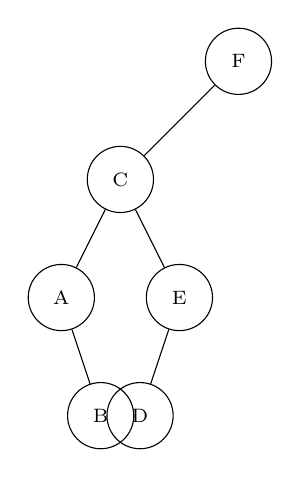
\begin{tikzpicture}[
every node/.style = {minimum width = 3em, draw, circle},
level/.style={sibling distance={3cm/max(1,#1)}}
]
\scriptsize
\node {F}
child{
node {C}
child {
node {A}
child[missing]
child{
node {B}
}
}
child {node {E}
child{
node {D}
}
child[missing]
}}
child[missing]
;
\end{tikzpicture}
\caption{\'Arbol generado por el algoritmo greedy}
\label{greedy}
\end{figure}
\end{document}
